% Created by tikzDevice version 0.12.4 on 2023-05-05 17:53:00
% !TEX encoding = UTF-8 Unicode
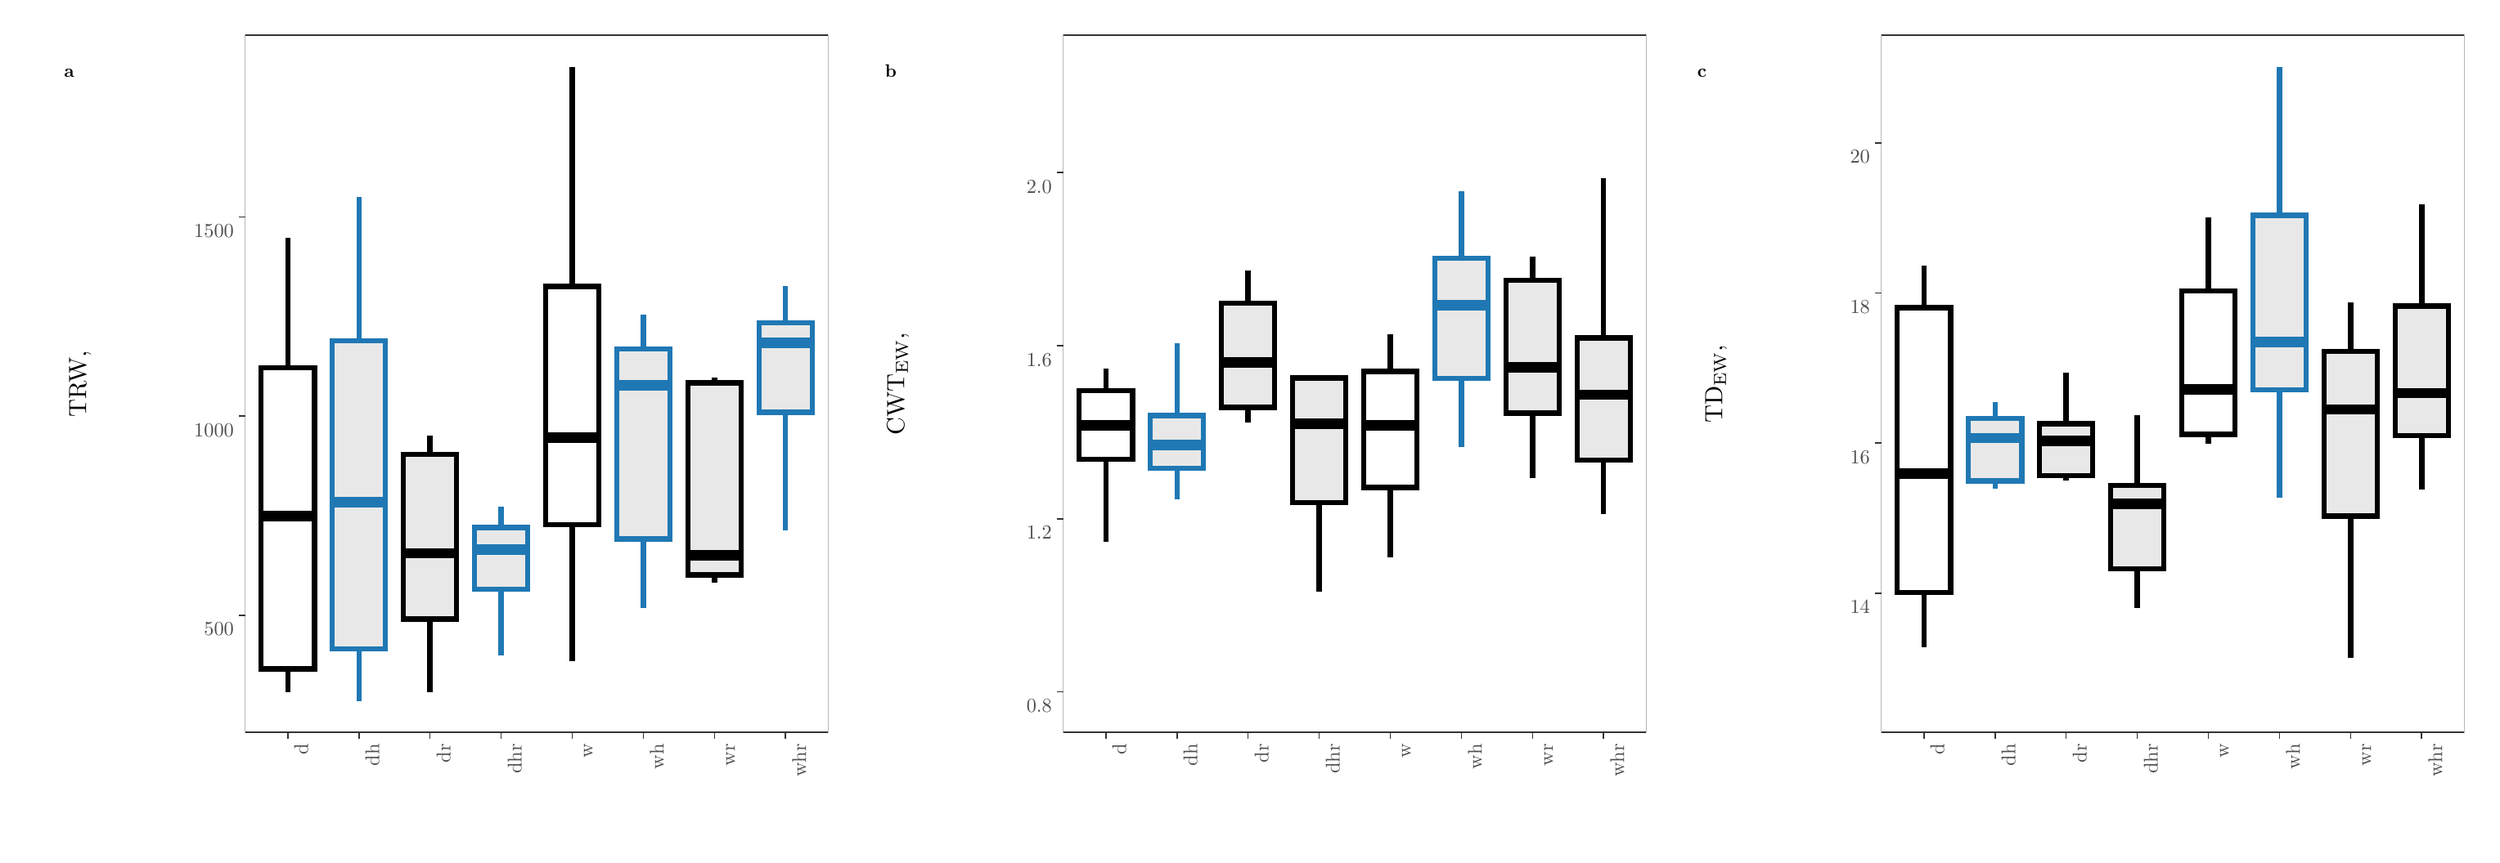
\begin{tikzpicture}[x=1pt,y=1pt]
\definecolor{fillColor}{RGB}{255,255,255}
\path[use as bounding box,fill=fillColor,fill opacity=0.00] (0,0) rectangle (1084.05,361.35);
\begin{scope}
\path[clip] (  0.00,  0.00) rectangle (361.35,361.35);
\definecolor{drawColor}{RGB}{255,255,255}
\definecolor{fillColor}{RGB}{255,255,255}

\path[draw=drawColor,line width= 0.6pt,line join=round,line cap=round,fill=fillColor] (  0.00,  0.00) rectangle (361.35,361.35);
\end{scope}
\begin{scope}
\path[clip] ( 98.25, 47.46) rectangle (355.85,355.85);
\definecolor{fillColor}{RGB}{255,255,255}

\path[fill=fillColor] ( 98.25, 47.46) rectangle (355.85,355.85);
\definecolor{drawColor}{RGB}{0,0,0}

\path[draw=drawColor,line width= 2.3pt,line join=round] (117.10,208.81) -- (117.10,266.22);

\path[draw=drawColor,line width= 2.3pt,line join=round] (117.10, 75.53) -- (117.10, 65.46);

\path[draw=drawColor,line width= 2.3pt,fill=fillColor] (105.32,208.81) --
	(105.32, 75.53) --
	(128.88, 75.53) --
	(128.88,208.81) --
	(105.32,208.81) --
	cycle;

\path[draw=drawColor,line width= 4.6pt] (105.32,143.08) -- (128.88,143.08);
\definecolor{drawColor}{RGB}{31,120,180}

\path[draw=drawColor,line width= 2.3pt,line join=round] (148.52,220.77) -- (148.52,284.34);

\path[draw=drawColor,line width= 2.3pt,line join=round] (148.52, 84.42) -- (148.52, 61.48);
\definecolor{fillColor}{RGB}{211,211,211}

\path[draw=drawColor,line width= 2.3pt,fill=fillColor,fill opacity=0.50] (136.74,220.77) --
	(136.74, 84.42) --
	(160.30, 84.42) --
	(160.30,220.77) --
	(136.74,220.77) --
	cycle;

\path[draw=drawColor,line width= 4.6pt] (136.74,149.26) -- (160.30,149.26);
\definecolor{drawColor}{RGB}{0,0,0}

\path[draw=drawColor,line width= 2.3pt,line join=round] (179.93,170.46) -- (179.93,178.57);

\path[draw=drawColor,line width= 2.3pt,line join=round] (179.93, 97.56) -- (179.93, 65.44);

\path[draw=drawColor,line width= 2.3pt,fill=fillColor,fill opacity=0.50] (168.15,170.46) --
	(168.15, 97.56) --
	(191.71, 97.56) --
	(191.71,170.46) --
	(168.15,170.46) --
	cycle;

\path[draw=drawColor,line width= 4.6pt] (168.15,126.75) -- (191.71,126.75);
\definecolor{drawColor}{RGB}{31,120,180}

\path[draw=drawColor,line width= 2.3pt,line join=round] (211.35,138.05) -- (211.35,147.30);

\path[draw=drawColor,line width= 2.3pt,line join=round] (211.35,110.74) -- (211.35, 81.69);

\path[draw=drawColor,line width= 2.3pt,fill=fillColor,fill opacity=0.50] (199.57,138.05) --
	(199.57,110.74) --
	(223.13,110.74) --
	(223.13,138.05) --
	(199.57,138.05) --
	cycle;

\path[draw=drawColor,line width= 4.6pt] (199.57,128.37) -- (223.13,128.37);
\definecolor{drawColor}{RGB}{0,0,0}

\path[draw=drawColor,line width= 2.3pt,line join=round] (242.76,244.75) -- (242.76,341.83);

\path[draw=drawColor,line width= 2.3pt,line join=round] (242.76,139.42) -- (242.76, 79.02);
\definecolor{fillColor}{RGB}{255,255,255}

\path[draw=drawColor,line width= 2.3pt,fill=fillColor] (230.98,244.75) --
	(230.98,139.42) --
	(254.54,139.42) --
	(254.54,244.75) --
	(230.98,244.75) --
	cycle;

\path[draw=drawColor,line width= 4.6pt] (230.98,177.93) -- (254.54,177.93);
\definecolor{drawColor}{RGB}{31,120,180}

\path[draw=drawColor,line width= 2.3pt,line join=round] (274.17,216.96) -- (274.17,232.11);

\path[draw=drawColor,line width= 2.3pt,line join=round] (274.17,133.10) -- (274.17,102.34);
\definecolor{fillColor}{RGB}{211,211,211}

\path[draw=drawColor,line width= 2.3pt,fill=fillColor,fill opacity=0.50] (262.39,216.96) --
	(262.39,133.10) --
	(285.95,133.10) --
	(285.95,216.96) --
	(262.39,216.96) --
	cycle;

\path[draw=drawColor,line width= 4.6pt] (262.39,200.98) -- (285.95,200.98);
\definecolor{drawColor}{RGB}{0,0,0}

\path[draw=drawColor,line width= 2.3pt,line join=round] (305.59,202.07) -- (305.59,204.50);

\path[draw=drawColor,line width= 2.3pt,line join=round] (305.59,117.09) -- (305.59,113.79);

\path[draw=drawColor,line width= 2.3pt,fill=fillColor,fill opacity=0.50] (293.81,202.07) --
	(293.81,117.09) --
	(317.37,117.09) --
	(317.37,202.07) --
	(293.81,202.07) --
	cycle;

\path[draw=drawColor,line width= 4.6pt] (293.81,125.81) -- (317.37,125.81);
\definecolor{drawColor}{RGB}{31,120,180}

\path[draw=drawColor,line width= 2.3pt,line join=round] (337.00,228.70) -- (337.00,244.87);

\path[draw=drawColor,line width= 2.3pt,line join=round] (337.00,189.04) -- (337.00,136.67);

\path[draw=drawColor,line width= 2.3pt,fill=fillColor,fill opacity=0.50] (325.22,228.70) --
	(325.22,189.04) --
	(348.78,189.04) --
	(348.78,228.70) --
	(325.22,228.70) --
	cycle;

\path[draw=drawColor,line width= 4.6pt] (325.22,219.89) -- (348.78,219.89);
\definecolor{drawColor}{gray}{0.20}

\path[draw=drawColor,line width= 0.6pt,line join=round,line cap=round] ( 98.25, 47.46) rectangle (355.85,355.85);
\end{scope}
\begin{scope}
\path[clip] (  0.00,  0.00) rectangle (1084.05,361.35);
\definecolor{drawColor}{gray}{0.30}

\node[text=drawColor,anchor=base east,inner sep=0pt, outer sep=0pt, scale=  0.88] at ( 93.30, 90.33) {500};

\node[text=drawColor,anchor=base east,inner sep=0pt, outer sep=0pt, scale=  0.88] at ( 93.30,178.34) {1000};

\node[text=drawColor,anchor=base east,inner sep=0pt, outer sep=0pt, scale=  0.88] at ( 93.30,266.36) {1500};
\end{scope}
\begin{scope}
\path[clip] (  0.00,  0.00) rectangle (1084.05,361.35);
\definecolor{drawColor}{gray}{0.20}

\path[draw=drawColor,line width= 0.6pt,line join=round] ( 95.50, 99.36) --
	( 98.25, 99.36);

\path[draw=drawColor,line width= 0.6pt,line join=round] ( 95.50,187.37) --
	( 98.25,187.37);

\path[draw=drawColor,line width= 0.6pt,line join=round] ( 95.50,275.38) --
	( 98.25,275.38);
\end{scope}
\begin{scope}
\path[clip] (  0.00,  0.00) rectangle (1084.05,361.35);
\definecolor{drawColor}{gray}{0.20}

\path[draw=drawColor,line width= 0.6pt,line join=round] (117.10, 44.71) --
	(117.10, 47.46);

\path[draw=drawColor,line width= 0.6pt,line join=round] (148.52, 44.71) --
	(148.52, 47.46);

\path[draw=drawColor,line width= 0.6pt,line join=round] (179.93, 44.71) --
	(179.93, 47.46);

\path[draw=drawColor,line width= 0.6pt,line join=round] (211.35, 44.71) --
	(211.35, 47.46);

\path[draw=drawColor,line width= 0.6pt,line join=round] (242.76, 44.71) --
	(242.76, 47.46);

\path[draw=drawColor,line width= 0.6pt,line join=round] (274.17, 44.71) --
	(274.17, 47.46);

\path[draw=drawColor,line width= 0.6pt,line join=round] (305.59, 44.71) --
	(305.59, 47.46);

\path[draw=drawColor,line width= 0.6pt,line join=round] (337.00, 44.71) --
	(337.00, 47.46);
\end{scope}
\begin{scope}
\path[clip] (  0.00,  0.00) rectangle (1084.05,361.35);
\definecolor{drawColor}{gray}{0.30}

\node[text=drawColor,rotate= 90.00,anchor=base east,inner sep=0pt, outer sep=0pt, scale=  0.88] at (126.13, 42.51) {d};

\node[text=drawColor,rotate= 90.00,anchor=base east,inner sep=0pt, outer sep=0pt, scale=  0.88] at (157.54, 42.51) {dh};

\node[text=drawColor,rotate= 90.00,anchor=base east,inner sep=0pt, outer sep=0pt, scale=  0.88] at (188.96, 42.51) {dr};

\node[text=drawColor,rotate= 90.00,anchor=base east,inner sep=0pt, outer sep=0pt, scale=  0.88] at (220.37, 42.51) {dhr};

\node[text=drawColor,rotate= 90.00,anchor=base east,inner sep=0pt, outer sep=0pt, scale=  0.88] at (251.79, 42.51) {w};

\node[text=drawColor,rotate= 90.00,anchor=base east,inner sep=0pt, outer sep=0pt, scale=  0.88] at (283.20, 42.51) {wh};

\node[text=drawColor,rotate= 90.00,anchor=base east,inner sep=0pt, outer sep=0pt, scale=  0.88] at (314.61, 42.51) {wr};

\node[text=drawColor,rotate= 90.00,anchor=base east,inner sep=0pt, outer sep=0pt, scale=  0.88] at (346.03, 42.51) {whr};
\end{scope}
\begin{scope}
\path[clip] (  0.00,  0.00) rectangle (1084.05,361.35);
\definecolor{drawColor}{RGB}{0,0,0}

\node[text=drawColor,rotate= 90.00,anchor=base,inner sep=0pt, outer sep=0pt, scale=  1.10] at ( 28.07,201.65) {TRW, \SI{}{\micro\metre}};

\node[text=drawColor,rotate= 90.00,anchor=base,inner sep=0pt, outer sep=0pt, scale=  1.10] at ( 39.95,201.65) {};
\end{scope}
\begin{scope}
\path[clip] (  0.00,  0.00) rectangle (1084.05,361.35);
\definecolor{drawColor}{RGB}{0,0,0}

\node[text=drawColor,anchor=base west,inner sep=0pt, outer sep=0pt, scale=  0.80] at ( 18.34,337.09) {\bfseries a};
\end{scope}
\begin{scope}
\path[clip] (361.35,  0.00) rectangle (722.70,361.35);
\definecolor{drawColor}{RGB}{255,255,255}
\definecolor{fillColor}{RGB}{255,255,255}

\path[draw=drawColor,line width= 0.6pt,line join=round,line cap=round,fill=fillColor] (361.35,  0.00) rectangle (722.70,361.35);
\end{scope}
\begin{scope}
\path[clip] (459.60, 47.46) rectangle (717.20,355.85);
\definecolor{fillColor}{RGB}{255,255,255}

\path[fill=fillColor] (459.60, 47.46) rectangle (717.20,355.85);
\definecolor{drawColor}{RGB}{0,0,0}

\path[draw=drawColor,line width= 2.3pt,line join=round] (478.45,198.68) -- (478.45,208.24);

\path[draw=drawColor,line width= 2.3pt,line join=round] (478.45,168.19) -- (478.45,131.78);

\path[draw=drawColor,line width= 2.3pt,fill=fillColor] (466.67,198.68) --
	(466.67,168.19) --
	(490.23,168.19) --
	(490.23,198.68) --
	(466.67,198.68) --
	cycle;

\path[draw=drawColor,line width= 4.6pt] (466.67,183.39) -- (490.23,183.39);
\definecolor{drawColor}{RGB}{31,120,180}

\path[draw=drawColor,line width= 2.3pt,line join=round] (509.87,187.54) -- (509.87,219.44);

\path[draw=drawColor,line width= 2.3pt,line join=round] (509.87,164.33) -- (509.87,150.62);
\definecolor{fillColor}{RGB}{211,211,211}

\path[draw=drawColor,line width= 2.3pt,fill=fillColor,fill opacity=0.50] (498.09,187.54) --
	(498.09,164.33) --
	(521.65,164.33) --
	(521.65,187.54) --
	(498.09,187.54) --
	cycle;

\path[draw=drawColor,line width= 4.6pt] (498.09,174.71) -- (521.65,174.71);
\definecolor{drawColor}{RGB}{0,0,0}

\path[draw=drawColor,line width= 2.3pt,line join=round] (541.28,237.24) -- (541.28,251.89);

\path[draw=drawColor,line width= 2.3pt,line join=round] (541.28,191.24) -- (541.28,184.50);

\path[draw=drawColor,line width= 2.3pt,fill=fillColor,fill opacity=0.50] (529.50,237.24) --
	(529.50,191.24) --
	(553.06,191.24) --
	(553.06,237.24) --
	(529.50,237.24) --
	cycle;

\path[draw=drawColor,line width= 4.6pt] (529.50,211.17) -- (553.06,211.17);

\path[draw=drawColor,line width= 2.3pt,line join=round] (572.70,204.20) -- (572.70,205.50);

\path[draw=drawColor,line width= 2.3pt,line join=round] (572.70,149.10) -- (572.70,109.58);

\path[draw=drawColor,line width= 2.3pt,fill=fillColor,fill opacity=0.50] (560.92,204.20) --
	(560.92,149.10) --
	(584.48,149.10) --
	(584.48,204.20) --
	(560.92,204.20) --
	cycle;

\path[draw=drawColor,line width= 4.6pt] (560.92,184.06) -- (584.48,184.06);

\path[draw=drawColor,line width= 2.3pt,line join=round] (604.11,207.13) -- (604.11,223.50);

\path[draw=drawColor,line width= 2.3pt,line join=round] (604.11,155.81) -- (604.11,124.81);
\definecolor{fillColor}{RGB}{255,255,255}

\path[draw=drawColor,line width= 2.3pt,fill=fillColor] (592.33,207.13) --
	(592.33,155.81) --
	(615.89,155.81) --
	(615.89,207.13) --
	(592.33,207.13) --
	cycle;

\path[draw=drawColor,line width= 4.6pt] (592.33,183.24) -- (615.89,183.24);
\definecolor{drawColor}{RGB}{31,120,180}

\path[draw=drawColor,line width= 2.3pt,line join=round] (635.52,257.26) -- (635.52,286.62);

\path[draw=drawColor,line width= 2.3pt,line join=round] (635.52,204.10) -- (635.52,173.75);
\definecolor{fillColor}{RGB}{211,211,211}

\path[draw=drawColor,line width= 2.3pt,fill=fillColor,fill opacity=0.50] (623.74,257.26) --
	(623.74,204.10) --
	(647.30,204.10) --
	(647.30,257.26) --
	(623.74,257.26) --
	cycle;

\path[draw=drawColor,line width= 4.6pt] (623.74,236.28) -- (647.30,236.28);
\definecolor{drawColor}{RGB}{0,0,0}

\path[draw=drawColor,line width= 2.3pt,line join=round] (666.94,247.41) -- (666.94,257.96);

\path[draw=drawColor,line width= 2.3pt,line join=round] (666.94,188.74) -- (666.94,159.90);

\path[draw=drawColor,line width= 2.3pt,fill=fillColor,fill opacity=0.50] (655.16,247.41) --
	(655.16,188.74) --
	(678.72,188.74) --
	(678.72,247.41) --
	(655.16,247.41) --
	cycle;

\path[draw=drawColor,line width= 4.6pt] (655.16,208.86) -- (678.72,208.86);

\path[draw=drawColor,line width= 2.3pt,line join=round] (698.35,221.99) -- (698.35,292.47);

\path[draw=drawColor,line width= 2.3pt,line join=round] (698.35,167.99) -- (698.35,144.22);

\path[draw=drawColor,line width= 2.3pt,fill=fillColor,fill opacity=0.50] (686.57,221.99) --
	(686.57,167.99) --
	(710.13,167.99) --
	(710.13,221.99) --
	(686.57,221.99) --
	cycle;

\path[draw=drawColor,line width= 4.6pt] (686.57,196.77) -- (710.13,196.77);
\definecolor{drawColor}{gray}{0.20}

\path[draw=drawColor,line width= 0.6pt,line join=round,line cap=round] (459.60, 47.46) rectangle (717.20,355.85);
\end{scope}
\begin{scope}
\path[clip] (  0.00,  0.00) rectangle (1084.05,361.35);
\definecolor{drawColor}{gray}{0.30}

\node[text=drawColor,anchor=base east,inner sep=0pt, outer sep=0pt, scale=  0.88] at (454.65, 56.41) {0.8};

\node[text=drawColor,anchor=base east,inner sep=0pt, outer sep=0pt, scale=  0.88] at (454.65,132.93) {1.2};

\node[text=drawColor,anchor=base east,inner sep=0pt, outer sep=0pt, scale=  0.88] at (454.65,209.45) {1.6};

\node[text=drawColor,anchor=base east,inner sep=0pt, outer sep=0pt, scale=  0.88] at (454.65,285.97) {2.0};
\end{scope}
\begin{scope}
\path[clip] (  0.00,  0.00) rectangle (1084.05,361.35);
\definecolor{drawColor}{gray}{0.20}

\path[draw=drawColor,line width= 0.6pt,line join=round] (456.85, 65.44) --
	(459.60, 65.44);

\path[draw=drawColor,line width= 0.6pt,line join=round] (456.85,141.96) --
	(459.60,141.96);

\path[draw=drawColor,line width= 0.6pt,line join=round] (456.85,218.48) --
	(459.60,218.48);

\path[draw=drawColor,line width= 0.6pt,line join=round] (456.85,295.00) --
	(459.60,295.00);
\end{scope}
\begin{scope}
\path[clip] (  0.00,  0.00) rectangle (1084.05,361.35);
\definecolor{drawColor}{gray}{0.20}

\path[draw=drawColor,line width= 0.6pt,line join=round] (478.45, 44.71) --
	(478.45, 47.46);

\path[draw=drawColor,line width= 0.6pt,line join=round] (509.87, 44.71) --
	(509.87, 47.46);

\path[draw=drawColor,line width= 0.6pt,line join=round] (541.28, 44.71) --
	(541.28, 47.46);

\path[draw=drawColor,line width= 0.6pt,line join=round] (572.70, 44.71) --
	(572.70, 47.46);

\path[draw=drawColor,line width= 0.6pt,line join=round] (604.11, 44.71) --
	(604.11, 47.46);

\path[draw=drawColor,line width= 0.6pt,line join=round] (635.52, 44.71) --
	(635.52, 47.46);

\path[draw=drawColor,line width= 0.6pt,line join=round] (666.94, 44.71) --
	(666.94, 47.46);

\path[draw=drawColor,line width= 0.6pt,line join=round] (698.35, 44.71) --
	(698.35, 47.46);
\end{scope}
\begin{scope}
\path[clip] (  0.00,  0.00) rectangle (1084.05,361.35);
\definecolor{drawColor}{gray}{0.30}

\node[text=drawColor,rotate= 90.00,anchor=base east,inner sep=0pt, outer sep=0pt, scale=  0.88] at (487.48, 42.51) {d};

\node[text=drawColor,rotate= 90.00,anchor=base east,inner sep=0pt, outer sep=0pt, scale=  0.88] at (518.89, 42.51) {dh};

\node[text=drawColor,rotate= 90.00,anchor=base east,inner sep=0pt, outer sep=0pt, scale=  0.88] at (550.31, 42.51) {dr};

\node[text=drawColor,rotate= 90.00,anchor=base east,inner sep=0pt, outer sep=0pt, scale=  0.88] at (581.72, 42.51) {dhr};

\node[text=drawColor,rotate= 90.00,anchor=base east,inner sep=0pt, outer sep=0pt, scale=  0.88] at (613.14, 42.51) {w};

\node[text=drawColor,rotate= 90.00,anchor=base east,inner sep=0pt, outer sep=0pt, scale=  0.88] at (644.55, 42.51) {wh};

\node[text=drawColor,rotate= 90.00,anchor=base east,inner sep=0pt, outer sep=0pt, scale=  0.88] at (675.96, 42.51) {wr};

\node[text=drawColor,rotate= 90.00,anchor=base east,inner sep=0pt, outer sep=0pt, scale=  0.88] at (707.38, 42.51) {whr};
\end{scope}
\begin{scope}
\path[clip] (  0.00,  0.00) rectangle (1084.05,361.35);
\definecolor{drawColor}{RGB}{0,0,0}

\node[text=drawColor,rotate= 90.00,anchor=base,inner sep=0pt, outer sep=0pt, scale=  1.10] at (389.42,201.65) {CWT\textsubscript{EW}, \SI{}{\micro\metre}};

\node[text=drawColor,rotate= 90.00,anchor=base,inner sep=0pt, outer sep=0pt, scale=  1.10] at (401.30,201.65) {};
\end{scope}
\begin{scope}
\path[clip] (  0.00,  0.00) rectangle (1084.05,361.35);
\definecolor{drawColor}{RGB}{0,0,0}

\node[text=drawColor,anchor=base west,inner sep=0pt, outer sep=0pt, scale=  0.80] at (380.95,337.09) {\bfseries b};
\end{scope}
\begin{scope}
\path[clip] (722.70,  0.00) rectangle (1084.05,361.35);
\definecolor{drawColor}{RGB}{255,255,255}
\definecolor{fillColor}{RGB}{255,255,255}

\path[draw=drawColor,line width= 0.6pt,line join=round,line cap=round,fill=fillColor] (722.70,  0.00) rectangle (1084.05,361.35);
\end{scope}
\begin{scope}
\path[clip] (820.95, 47.46) rectangle (1078.55,355.85);
\definecolor{fillColor}{RGB}{255,255,255}

\path[fill=fillColor] (820.95, 47.46) rectangle (1078.55,355.85);
\definecolor{drawColor}{RGB}{0,0,0}

\path[draw=drawColor,line width= 2.3pt,line join=round] (839.80,235.25) -- (839.80,253.89);

\path[draw=drawColor,line width= 2.3pt,line join=round] (839.80,109.28) -- (839.80, 85.04);

\path[draw=drawColor,line width= 2.3pt,fill=fillColor] (828.02,235.25) --
	(828.02,109.28) --
	(851.58,109.28) --
	(851.58,235.25) --
	(828.02,235.25) --
	cycle;

\path[draw=drawColor,line width= 4.6pt] (828.02,162.07) -- (851.58,162.07);
\definecolor{drawColor}{RGB}{31,120,180}

\path[draw=drawColor,line width= 2.3pt,line join=round] (871.22,186.23) -- (871.22,193.70);

\path[draw=drawColor,line width= 2.3pt,line join=round] (871.22,158.70) -- (871.22,155.40);
\definecolor{fillColor}{RGB}{211,211,211}

\path[draw=drawColor,line width= 2.3pt,fill=fillColor,fill opacity=0.50] (859.44,186.23) --
	(859.44,158.70) --
	(883.00,158.70) --
	(883.00,186.23) --
	(859.44,186.23) --
	cycle;

\path[draw=drawColor,line width= 4.6pt] (859.44,177.66) -- (883.00,177.66);
\definecolor{drawColor}{RGB}{0,0,0}

\path[draw=drawColor,line width= 2.3pt,line join=round] (902.63,183.96) -- (902.63,206.51);

\path[draw=drawColor,line width= 2.3pt,line join=round] (902.63,160.98) -- (902.63,158.83);

\path[draw=drawColor,line width= 2.3pt,fill=fillColor,fill opacity=0.50] (890.85,183.96) --
	(890.85,160.98) --
	(914.41,160.98) --
	(914.41,183.96) --
	(890.85,183.96) --
	cycle;

\path[draw=drawColor,line width= 4.6pt] (890.85,176.46) -- (914.41,176.46);

\path[draw=drawColor,line width= 2.3pt,line join=round] (934.05,156.66) -- (934.05,187.63);

\path[draw=drawColor,line width= 2.3pt,line join=round] (934.05,119.87) -- (934.05,102.59);

\path[draw=drawColor,line width= 2.3pt,fill=fillColor,fill opacity=0.50] (922.27,156.66) --
	(922.27,119.87) --
	(945.83,119.87) --
	(945.83,156.66) --
	(922.27,156.66) --
	cycle;

\path[draw=drawColor,line width= 4.6pt] (922.27,148.59) -- (945.83,148.59);

\path[draw=drawColor,line width= 2.3pt,line join=round] (965.46,242.77) -- (965.46,275.38);

\path[draw=drawColor,line width= 2.3pt,line join=round] (965.46,179.24) -- (965.46,175.29);
\definecolor{fillColor}{RGB}{255,255,255}

\path[draw=drawColor,line width= 2.3pt,fill=fillColor] (953.68,242.77) --
	(953.68,179.24) --
	(977.24,179.24) --
	(977.24,242.77) --
	(953.68,242.77) --
	cycle;

\path[draw=drawColor,line width= 4.6pt] (953.68,199.28) -- (977.24,199.28);
\definecolor{drawColor}{RGB}{31,120,180}

\path[draw=drawColor,line width= 2.3pt,line join=round] (996.87,276.10) -- (996.87,341.83);

\path[draw=drawColor,line width= 2.3pt,line join=round] (996.87,199.03) -- (996.87,151.17);
\definecolor{fillColor}{RGB}{211,211,211}

\path[draw=drawColor,line width= 2.3pt,fill=fillColor,fill opacity=0.50] (985.09,276.10) --
	(985.09,199.03) --
	(1008.65,199.03) --
	(1008.65,276.10) --
	(985.09,276.10) --
	cycle;

\path[draw=drawColor,line width= 4.6pt] (985.09,220.09) -- (1008.65,220.09);
\definecolor{drawColor}{RGB}{0,0,0}

\path[draw=drawColor,line width= 2.3pt,line join=round] (1028.29,215.86) -- (1028.29,237.51);

\path[draw=drawColor,line width= 2.3pt,line join=round] (1028.29,143.13) -- (1028.29, 80.64);

\path[draw=drawColor,line width= 2.3pt,fill=fillColor,fill opacity=0.50] (1016.51,215.86) --
	(1016.51,143.13) --
	(1040.07,143.13) --
	(1040.07,215.86) --
	(1016.51,215.86) --
	cycle;

\path[draw=drawColor,line width= 4.6pt] (1016.51,190.31) -- (1040.07,190.31);

\path[draw=drawColor,line width= 2.3pt,line join=round] (1059.70,236.05) -- (1059.70,280.83);

\path[draw=drawColor,line width= 2.3pt,line join=round] (1059.70,178.81) -- (1059.70,154.87);

\path[draw=drawColor,line width= 2.3pt,fill=fillColor,fill opacity=0.50] (1047.92,236.05) --
	(1047.92,178.81) --
	(1071.48,178.81) --
	(1071.48,236.05) --
	(1047.92,236.05) --
	cycle;

\path[draw=drawColor,line width= 4.6pt] (1047.92,197.58) -- (1071.48,197.58);
\definecolor{drawColor}{gray}{0.20}

\path[draw=drawColor,line width= 0.6pt,line join=round,line cap=round] (820.95, 47.46) rectangle (1078.55,355.85);
\end{scope}
\begin{scope}
\path[clip] (  0.00,  0.00) rectangle (1084.05,361.35);
\definecolor{drawColor}{gray}{0.30}

\node[text=drawColor,anchor=base east,inner sep=0pt, outer sep=0pt, scale=  0.88] at (816.00,100.07) {14};

\node[text=drawColor,anchor=base east,inner sep=0pt, outer sep=0pt, scale=  0.88] at (816.00,166.44) {16};

\node[text=drawColor,anchor=base east,inner sep=0pt, outer sep=0pt, scale=  0.88] at (816.00,232.81) {18};

\node[text=drawColor,anchor=base east,inner sep=0pt, outer sep=0pt, scale=  0.88] at (816.00,299.18) {20};
\end{scope}
\begin{scope}
\path[clip] (  0.00,  0.00) rectangle (1084.05,361.35);
\definecolor{drawColor}{gray}{0.20}

\path[draw=drawColor,line width= 0.6pt,line join=round] (818.20,109.09) --
	(820.95,109.09);

\path[draw=drawColor,line width= 0.6pt,line join=round] (818.20,175.47) --
	(820.95,175.47);

\path[draw=drawColor,line width= 0.6pt,line join=round] (818.20,241.84) --
	(820.95,241.84);

\path[draw=drawColor,line width= 0.6pt,line join=round] (818.20,308.21) --
	(820.95,308.21);
\end{scope}
\begin{scope}
\path[clip] (  0.00,  0.00) rectangle (1084.05,361.35);
\definecolor{drawColor}{gray}{0.20}

\path[draw=drawColor,line width= 0.6pt,line join=round] (839.80, 44.71) --
	(839.80, 47.46);

\path[draw=drawColor,line width= 0.6pt,line join=round] (871.22, 44.71) --
	(871.22, 47.46);

\path[draw=drawColor,line width= 0.6pt,line join=round] (902.63, 44.71) --
	(902.63, 47.46);

\path[draw=drawColor,line width= 0.6pt,line join=round] (934.05, 44.71) --
	(934.05, 47.46);

\path[draw=drawColor,line width= 0.6pt,line join=round] (965.46, 44.71) --
	(965.46, 47.46);

\path[draw=drawColor,line width= 0.6pt,line join=round] (996.87, 44.71) --
	(996.87, 47.46);

\path[draw=drawColor,line width= 0.6pt,line join=round] (1028.29, 44.71) --
	(1028.29, 47.46);

\path[draw=drawColor,line width= 0.6pt,line join=round] (1059.70, 44.71) --
	(1059.70, 47.46);
\end{scope}
\begin{scope}
\path[clip] (  0.00,  0.00) rectangle (1084.05,361.35);
\definecolor{drawColor}{gray}{0.30}

\node[text=drawColor,rotate= 90.00,anchor=base east,inner sep=0pt, outer sep=0pt, scale=  0.88] at (848.83, 42.51) {d};

\node[text=drawColor,rotate= 90.00,anchor=base east,inner sep=0pt, outer sep=0pt, scale=  0.88] at (880.24, 42.51) {dh};

\node[text=drawColor,rotate= 90.00,anchor=base east,inner sep=0pt, outer sep=0pt, scale=  0.88] at (911.66, 42.51) {dr};

\node[text=drawColor,rotate= 90.00,anchor=base east,inner sep=0pt, outer sep=0pt, scale=  0.88] at (943.07, 42.51) {dhr};

\node[text=drawColor,rotate= 90.00,anchor=base east,inner sep=0pt, outer sep=0pt, scale=  0.88] at (974.49, 42.51) {w};

\node[text=drawColor,rotate= 90.00,anchor=base east,inner sep=0pt, outer sep=0pt, scale=  0.88] at (1005.90, 42.51) {wh};

\node[text=drawColor,rotate= 90.00,anchor=base east,inner sep=0pt, outer sep=0pt, scale=  0.88] at (1037.31, 42.51) {wr};

\node[text=drawColor,rotate= 90.00,anchor=base east,inner sep=0pt, outer sep=0pt, scale=  0.88] at (1068.73, 42.51) {whr};
\end{scope}
\begin{scope}
\path[clip] (  0.00,  0.00) rectangle (1084.05,361.35);
\definecolor{drawColor}{RGB}{0,0,0}

\node[text=drawColor,rotate= 90.00,anchor=base,inner sep=0pt, outer sep=0pt, scale=  1.10] at (750.77,201.65) {TD\textsubscript{EW}, \SI{}{\micro\metre}};

\node[text=drawColor,rotate= 90.00,anchor=base,inner sep=0pt, outer sep=0pt, scale=  1.10] at (762.65,201.65) {};
\end{scope}
\begin{scope}
\path[clip] (  0.00,  0.00) rectangle (1084.05,361.35);
\definecolor{drawColor}{RGB}{0,0,0}

\node[text=drawColor,anchor=base west,inner sep=0pt, outer sep=0pt, scale=  0.80] at (739.78,337.09) {\bfseries c};
\end{scope}
\end{tikzpicture}
